\documentclass[14pt]{article}
\usepackage{amsmath,amsthm,amsfonts,amssymb,tikz,scalerel,mathrsfs,marvosym,titlesec,leftidx}

\usepackage{tikz}
\def\layersep{2.5cm}
\usepackage[all]{xy}
\usepackage{fancyhdr}
\usepackage{blkarray}
\usepackage{adjustbox}
\usepackage{hyperref}
\usepackage[linesnumbered,ruled]{algorithm2e}


\usepackage[font=small,labelfont=bf,tableposition=top]{caption}



\DeclareCaptionLabelFormat{andtable}{#1~#2  \&  \tablename~\thetable}

\theoremstyle{plain}
\newtheorem{corollary}{Corollary}[subsection]
\newtheorem{convention}[corollary]{Convention}
\newtheorem{example}[corollary]{Example}
\newtheorem*{theorem*}{theorem}
\newtheorem{theorem}[corollary]{Theorem}
\newtheorem{lemma}[corollary]{Lemma}
\newtheorem*{lemma*}{Lemma}
\newtheorem{maintheorem}{Theorem}
%reset maintheorem counter to use the corresponding letter
\renewcommand{\themaintheorem}{\Alph{maintheorem}}
\newtheorem{remark}[corollary]{Remark}
\newtheorem{proposition}[corollary]{Proposition}


\theoremstyle{definition}
\newtheorem{definition}[corollary]{Definition}
\newtheorem{definition*}{Definition}

%change the default font to bodoni
\usepackage[default]{gfsbodoni}
\usepackage[T1]{fontenc}



%start at section 0 for introduction 
\setcounter{section}{-1}
\newcommand{\un}{\textunderscore}
\newcommand{\A}{\mathcal{A}}
\newcommand{\abs}[1]{\vert #1 \vert }
\DeclareMathOperator{\ad}{ad}
\DeclareMathOperator{\Aut}{Aut}
\renewcommand{\b}{\bullet}
\newcommand{\bp}{\mathbf{\Pi}}
\newcommand{\bl}[2]{\left\langle #1,#2\right\rangle}
\def\BVm{\operatorname{BV}_-}
\DeclareMathOperator{\BiMod}{BiMod}
\DeclareMathOperator{\bimod}{bimod}
\newcommand{\C}{{\mathcal{C}}}
\DeclareMathOperator{\CC}{CC}
\def\cd{\operatorname {cd}}
\DeclareMathOperator{\ch}{ch}
\DeclareMathOperator{\CH}{CH}
\DeclareMathOperator{\coh}{coh}
\DeclareMathOperator{\cone}{cone}
\DeclareMathOperator{\coker}{coker}
\renewcommand{\d}[1]{\mathbb{#1}}
\newcommand{\D}{{\mathscr{D}}}
\DeclareMathOperator{\der}{R}
\DeclareMathOperator{\Def}{Def}
\newcommand{\define}{\stackrel{\operatorname{def}}{=}}
\let\div\relax %unassign \div
\DeclareMathOperator{\div}{div}
\DeclareMathOperator{\divu}{div}
\newcommand{\ds}{\oplus}
\newcommand{\DS}{\bigoplus}
\newcommand{\epi}{\xymatrix{{}\ar@{->>}[r]&{}}}
\DeclareMathOperator{\End}{End}
\DeclareMathOperator{\Ext}{Ext}
\newcommand{\f}[1]{\mathfrak{#1}}
\DeclareMathOperator{\fd}{fd}
\newcommand{\fC}{\f{C}}
\newcommand{\fD}{\f{D}}
\newcommand{\floor}[1]{\left\lfloor #1 \right\rfloor}
\newcommand{\fun}{\mapsto}
\newcommand{\dgg}{{\f{g}^\bullet}}
\newcommand{\g}{\f{g}}
\DeclareMathOperator{\Gd}{Gd}
\DeclareMathOperator{\Gr}{Gr}
\DeclareMathOperator{\gldim}{gl.dim}
\let\H\relax %unassign \H
\DeclareMathOperator{\H}{H}
\DeclareMathOperator{\HH}{HH}
\DeclareMathOperator{\HC}{HC}
\DeclareMathOperator{\Hom}{Hom}
\DeclareMathOperator{\Id}{Id}
\DeclareMathOperator{\im}{im}
\newcommand{\iso}{\stackrel{\sim}{\longrightarrow}}
\DeclareMathOperator{\Jac}{Jac}
\renewcommand{\k}{\Bbbk}
\newcommand{\K}{\mathbb{K}}
\DeclareMathOperator{\length}{length}
\DeclareMathOperator{\lrk}{\l.rk}
\newcommand{\leftperp}[1]{\leftidx{^\perp}{#1}}
\newcommand{\m}{\f{m}}
\DeclareMathOperator{\MCM}{MCM}
\DeclareMathOperator{\MC}{MC}
\DeclareMathOperator{\MCcal}{\mathcal{MC}}
\DeclareMathOperator{\Mod}{Mod}
\DeclareMathOperator{\Mor}{Mor}
\def\mod{\operatorname{mod}}
\newcommand{\mor}{\longrightarrow}
\DeclareMathOperator{\Test}{Test}
\newcommand{\T}{\mathscr{T}}
\renewcommand{\O}{\mathcal{O}}
\DeclareMathOperator{\NS}{NS}
\DeclareMathOperator{\Num}{Num}
\newcommand{\p}{\mathfrak{p}}
\DeclareMathOperator{\per}{per}
\DeclareMathOperator{\Ob}{Ob}
\DeclareMathOperator{\Perf}{Perf}
\DeclareMathOperator{\Pic}{Pic}
\DeclareMathOperator{\Proj}{Proj}
\DeclareMathOperator{\poly}{poly}
\DeclareMathOperator{\Qcoh}{Qcoh}
\DeclareMathOperator{\QGr}{QGr}
\DeclareMathOperator{\RHom}{RHom}
\renewcommand{\r}[1]{\mathcal{#1}}
\DeclareMathOperator{\rk}{rk}
\DeclareMathOperator{\rrk}{r.rk}
\def\locExt{\mathscr{E}\mathit{xt}}
\DeclareMathOperator{\SL}{SL}
\DeclareMathOperator{\SPS}{SPS}
\DeclareMathOperator{\sing}{sing}
\DeclareMathOperator{\vectorspan}{span}
\DeclareMathOperator{\Spec}{Spec}
\DeclareMathOperator{\Supp}{Supp}
\DeclareMathOperator{\SupVec}{SupVec}
\DeclareMathOperator{\Sym}{Sym}
\def\locHom{\operatorname {\mathscr{H}\mathit{om}}}
\DeclareMathOperator{\Tails}{Tails}
\def\ltr{\overset{L}{\tr}}
\renewcommand{\r}[1]{\mathcal{#1}}
\newcommand{\mono}{\xymatrix{{}\ar@{^{(}->}[r]&{}}}\DeclareMathOperator{\num}{num}
\DeclareMathOperator{\rad}{rad}
\DeclareMathOperator{\Tor}{Tor}
\DeclareMathOperator{\Tors}{Tors}
\newcommand{\tr}{\otimes}
\newcommand{\trps}[1]{ \leftidx{^{\operatorname{tr}}}{#1}}
\def\uRHom{\operatorname {R\mathcal{H}\mathit{om}}}
\newcommand{\w}{{\tt{w}}}
\newcommand{\Q}{\mathbb{Q}}
\DeclareMathOperator{\qis}{qis}
\DeclareMathOperator{\Qvr}{\mathcal{Q}}
\newcommand{\Z}{\mathbb{Z}}


%add dots between section and page in toc
\usepackage{tocloft}
\renewcommand{\cftsecleader}{\cftdotfill{\cftdotsep}}


%interline a little larger
\linespread{1.28}

%change the dimensions of the margin
\usepackage{geometry}
 \geometry{
 a4paper,
 total={210mm,297mm},
 left=23mm,
 right=23mm,
 top=32mm,
 bottom=20mm,
 }
 
%changeqedsymbol
\renewcommand{\qedsymbol}{\CrossedBox}

%make the (sub)subsections run into the text, the 0.25 is the distance between the numbering and title
\titleformat{\subsubsection}[runin]{\normalfont\normalsize\bfseries}{\thesubsubsection.}{0.25em}{}
\begin{document}
\title{\textbf{CAPSTONE PROJECT: DECTECING FORGED BANKNOTES}}
\author{LOUIS DE THANHOFFER DE VOLCSEY}
\date{\emph{september 2017}}
\maketitle	
\vspace{1in}
%add header on other pages

\pagestyle{fancy}
\lhead{Capstone Project} \rhead{L. de Thanhoffer}
\chead{{\large{\bf Detecting Counterfeit Banknotes}}} \lfoot{} \rfoot{\bf  page \thepage} \cfoot{}

\noindent\hrulefill
\tableofcontents{}
\noindent\hrulefill
\newpage 
\section{Introduction}
\subsection{Overview}
In this project we design a neural net capable of reliably detecting forged banknotes.\\ Our algorithm relies on data that was collected by scanning notes which were subsequently processed statistically through a mathematical operation called a \emph{wavelet transform}. In doing this, one is able to distill some of the key features that describe the inherent mathematical information inherent to each image.\\ 
Our approach can be subdivided in two major steps:
\begin{enumerate}
\item {\bf reingineering the data}. Based on the famous machine learning folklore:
\begin{center}
\emph{95\% of machine learning is feature engineering}	
\end{center}
we will first perform an analysis of the data and manipulate it in order to optimize it  before fitting it to a neural network. 
Some of the techniques we use include:  detecting and removing outliers, describing the various relations between different features, reducing the dimension of the data to 3 and 2 as well as analyzing to what extend the data can be separated linearly.
\item
{\bf Designing a neural network}
Once the data has been reengineered, we use the \texttt{keras} library to implement an optimal neural net. To this end, we initially consider a rather simple model and analyze its performance through the use of learning curves. These curves give us not only an insight into how accurate the neural net is, but allow us to understand how to adapt the design in order to improve the accuracy. Our final model will result in a model capable of accurately detecting forged banknotes 98\% of the time all the while retaining a simple and transparent architecture.
\end{enumerate}
\subsection{Background to the problem}
Know colloquially as one of the \emph{worlds second oldest profession} \cite{wikiprof}, the art of counterfeiting legal tender dates back to the invention of money itself. From forgers reproducing gold coins in Roman times by using cheaper base metals \cite{wikiforge} to the use of Mulberry trees \cite{wikiforge} in order to imitate banknotes in 13th century China, forgers and governments have always played a fiendish cat-and-mouse game that makes for a fascinating history. Counterfeiting techniques were even used as a form of warfare in the U.S. Revolutionary war by the British in order to devaluate the newly created U.S. dollar \cite{wikiforge}.\\
The problem of counterfeiting however, is not just one of historical importance. In fact, it is estimated that this issue produces an annual increase in inflation resulting in a loss of purchasing power of about  250 billion dollar annually for the U.S. economy \cite{usforge}.\\ 
In  modern times, the techniques to detect forgery have grown very subtle as anti-counterfeiting measures enter the 21st century. The main paradigm behind these techniques has however remained unchanged after centuries: from the use of complicated printing techniques to the inclusion of watermarks- at its core, a note is fitted with a set of attributes and ran through a subsequent series of tests (some by hand, some automatic) to determine if those attributes are indeed present in the banknote.\\ \\This project aims to detect forgery in a different way. Instead, using mathematical analysis, the banknote will inherently be described in waveform. We will subsequently use the machinery of neural networks to infer a formula which uses some inherent statistical features of this wave allowing us to detect forgery.

\section{Analyzing the dataset}
The dataset in question was extracted from the UC Irvine machine learning repository \footnote{\url{https://archive.ics.uci.edu/ml/datasets/banknote+authentication}}. It serves as the basis for a regression analysis performed by Gillich and Lowesh in \cite{BNA}. In loc. sit. the authors first scanned a set of 1372 banknotes into 400$\times$ 400 pixel images. Subsequently, to each image, a \emph{Wavelet transform} was applied. This is a mathematical tools which finds its origins in the theory of Fourier transforms and allows one to encode the image data very efficiently. For our purposes it will be sufficient to know that it compresses an image by extracting coefficients which according to an underlying probability distribution. The features of the dataset in question consists of a description of 4 statistical properties of this distribution:
\begin{enumerate}
\item the variance
\item the skewness
\item the kurtosis	
\item the Shannon entropy
\end{enumerate}
Finally, to each feature a binary target label is associated indicating whether the note is real or counterfeit. In the dataset, the first 762 notes are real, whereas the last 610 are counterfeit. By way of example, the 350'th datapoint is the $5$-tuple:

\begin{center}
\texttt{[-1.5768,10.843,2.5462,-2.9362,0]
}	
\end{center}
\subsection{a First exploration}
We begin by describing the basic statistical properties of the data. These are listed below as well as displayed graphically in the form of a boxplot:
\begin{table}[ht]
\begin{minipage}[b]{0.56\linewidth}
\centering
\begin{tabular}{|c| c| c |c |c|}
\hline
\texttt{statistic} & \texttt{variance} &\texttt{skewness}&\texttt{curtosis}  &\texttt{entropy} \\
	\hline
         mean &    0.43 &   1.92 &   1.40  & -1.19\\
         \hline
         std  &    2.84  &   5.87  &   4.31   &  2.10\\
         \hline
         min  &    -7.042 & -13.77  & -5.29    & -8.55\\
         \hline
         25\% &   -1.77  &  -1.71  &   -1.57  & -2.41\\
         \hline
         50\% &   0.50 &  2.32   &  0.62    &  -0.59\\
         \hline
         75\% &   2.82   &  6.81   &  3.18    &  0.39\\
         \hline
         max  &    6.82  &  12.95  &  17.93   &  2.45\\
         \hline
 \end{tabular}   
 \caption{describing the data}
    \label{table:student}
\end{minipage}\hfill
\begin{minipage}[b]{0.4\linewidth}
\centering
\includegraphics[width=67mm]{banknote_forgery_files/banknote_forgery_9_0}
\captionof{figure}{the boxplot of the data}
\label{boxplot}
\end{minipage}
\end{table}

We see that all $4$ features have rather similar statistical properties. As such we choose to not renormalize the data.\\ 
One  observation to be made is that a there seems to be a significant number of datapoints whose kurtosis have a value above the boxplot whiskers. These should be considered outliers. Similarly, a number of datapoint are outliers for the entropy feature. After counting these in numpy, we removed a total of {\bf 65} datapoints (equivalent to {\bf 4.3\%} of the total data).\\ 
The new dataset now consist of {\bf 1305} entries and has no outliers.
\subsection{the Correlation between features} The next step in our data exploration, consists of investigation any possible correlations between features. This is an important step as correlated features morally correspond to redundant information, which may cause overfitting as we build a classifier. The Pearson correlation coefficients are listed in the table below, together with the scatterplots of all possible choices of features \footnote{we note that in the case where two identical features are chosen, their histogram is displayed}
\begin{table}[ht]
\begin{minipage}[b]{0.4\linewidth}
\centering
\begin{tabular}{|c |c| c| c |c |}
\hline
feature  &         var   &   skew &     curt    &   ent\\
  \hline
var &   1 & 0.26 & -0.38 & 0.27\\
\hline
skew & 0.26 & 1 & -0.78 & -0.52\\
\hline
curt & -0.38 & -0.78 &  1  & 0.32\\
\hline
ent   & 0.27 & -0.52 &  0.32 &  1\\
\hline
\end{tabular}
\vspace{0.83in}
 \caption{the Pearson correlation matrix}
    \label{table:student}
\end{minipage}
\begin{minipage}[b]{0.445\linewidth}
\centering
\includegraphics[width=95mm]{banknote_forgery_files/banknote_forgery_15_1}
\captionof{figure}{the scatterplot of the features}
\label{boxplot}
\end{minipage}
\end{table}

 Both the Pearson table and the scatterplot indicate that exactly two features are significantly correlated: kurtosis and skewness have a Pearson correlation of 78\% in absolute value. Additionally, the scatterplot shows that linear trend seems to form around $y=-x$ between those features.\\ 
 We choose however to keep both those features as this this would significantly reduce the dataspace which could impact the predictive capabilities performance of the final model. Instead, since the learning accuracy of each model will be represented through a learning curve at a later stage we will be able to detect any overfitting behavior at that stage and adapt the model accordingly. 

\subsection{Reducing the dimension} The third step next step in our analysis consists of reducing the dimension of the data from $4$ to $3$ and $2$ subsequently. The method of choice for such problems is a principal component analysis, in which one first determines an optimal subspace by maximizing the variance (or equivalently minimizing the mean square error), exhibits an orthonormal basis for this subspace and subsequently computes the coordinate for any projected vector with respect to this basis. For the reader's benefit. A pseudo-algorithm of this procedure in sklearn is given below: 
\newpage 
\begin{algorithm}\label{PCAalg}
    \SetKwInOut{Input}{Input}
    \SetKwInOut{Output}{Output}

    \underline{function reduce} $(\textrm{features}, d)$\;
    \Input{a set of features, together with the desired final dimension}
    \Output{a new set of dimension $d$, together with the total variance of each dimension}
    pca=PCA(n\textunderscore features=$d$) \\
  	pca.fit(features)\\
    print(pca.explained\textunderscore variance\textunderscore ratio\textunderscore	\\
   reduced\textunderscore data=pca.transform(new\textunderscore features)\\
   return reduced\un data      
   \caption{reduce dimensionality using PCA }
\end{algorithm}
The total variation in each component after applying a PCA transformation is listed below:\\
\begin{center}
\begin{tabular}{|c|c|c|c|c|}
	\hline
	component & 1 & 2 & 3& 4\\
	\hline
	expl. var.& 76\%&  14\% & 6\% & 3\%\\
	 \hline
\end{tabular}
\end{center}
    
   
    
\subsection{Plotting the data} Reducing the dataset allows us to observe how the binary labels are distributed in the dataset in a scatterplot.\\ In the figures below, the reduced data (following \ref{PCAalg} are pictured. The red labels correspond to real banknotes, whereas the green labels represent forgeries.

\begin{table}[ht]
\begin{minipage}[b]{0.56\linewidth}
\centering
\includegraphics[width=90mm]{banknote_forgery_files/model_1}
 \caption{the 3d reduced data}
    \label{table:student}
\end{minipage}\hfill
\begin{minipage}[b]{0.4\linewidth}
\centering
\includegraphics[width=70mm]{banknote_forgery_files/model_2}
\vspace{0.29in}
\captionof{figure}{the 2d reduced data}
\label{boxplot}
\end{minipage}
\end{table}

These plots indicate that the reduced data is not linearly separable. This hypothesis can be confirmed numerically through the use of a support vector machine. This clustering tool finds a hyperplane that maximizes the marginal distance between the hyperplane in question and the two different classes of points. In the algorithm below, we use the \texttt{reduce} function described earlier, fit a support vector machine and compute the accuracy of this classifier -which in this case simply the relative number of misclassified points:
     \begin{algorithm}
    \SetKwInOut{Input}{Input}
    \SetKwInOut{Output}{Output}

    \underline{function lin \un sep\un acc} $(\textrm{features},m)$\;
    \Input{a set of features}
    \Output{the accuracy of a separating hyperplane after reducing dimensions up to $m$}
    d=features.shape[1]\\
    \For{i in range(\textrm{m,d+1}) }{reduced\un features=reduce(features,$i$)\\

    	clf=SVC()\\
		clf.fit(reduced\un features,labels)\\
		predicted\un labels=clf.predict(reduced\un features)\\
		accuracy\un score(predicted\un labels,labels)\\
		}      
   \caption{compute the accuracy of a separating hyperplane after reducing dimensions}
\end{algorithm}
The results of this algorithm are listed in the table below:
\begin{center}
\begin{tabular}{|c|c|c|c|}
	\hline
	dimension & 4 & 3 & 2\\ 
	\hline 
	accuracy & 81\% & 78\% & 59\%\\
	\hline
\end{tabular}
\end{center}
  This indeed confirms our hypothesis that the data cannot be linearly separated, even after reducing dimensions. It is worth noting that one could alternatively implement a support vector machine with a more sophisticated kernel. This would result in a slightly more appropriate decision boundary and a higher accuracy as a result. However, since the data does not visually seem to have obvious decision boundary. It is likely that this accuracy would be a result of overfitting.
\subsection{Conclusions}
Our analysis of the data has let us to the following conclusions:
\begin{itemize}
\item The dataset -consisting of $4$ features with binary labels-  is roughly equidistributed. As such  we do not perform any rescaling operation in order to keep transparency.
\item A closer look does show outliers however. After removing these 95.7\% of the mass is retained.
\item Within the data, two features are heavily correlated: computing the Pearson coefficient of kurtosis vs. skewness results in a $\vert 72\%\vert $ correlation. This could be a possible explanation of overfitting later on.
\item Applying a principal component analysis allows us to reduce the data to 3 or 2 dimensions and to conclude that the distribution of the labels is rather heterogeneous. In particular the data does not present an obvious decision boundary.
\item Fitting a support vector machine (after reducing the dimensions) supports this evidence. In fact, classifying the labels using a separating hyperplane results in misclassification about 20\% of the time.
\end{itemize}

\newpage
\section{Building a neural net}
The previous section allowed us to conclude that the data may be prone to overfitting and that a simple decision boundary does not exist. In light of these facts, we opt to use a neural network to classify the data, as these are robust enough to handle more complicated data all the while remaining transparent in their design.
\subsection{Neural nets in Keras} 

To implement and optimize a neural net, we will  use the \texttt{keras} Python library using a \texttt{TensorFlow} backend. This library (built specifically for neural networks) has become one of the gold standards in the industry due to its ease of use and modularity.\\
In fact, the programming paradigm in \texttt{keras} is remarkably streamlined. Essentially, a network is built in two steps:
\begin{enumerate}
\item One first designs the net layer by layer. For each layer the user can easily specify the number of input nodes, the activation function or use or implement regularization functionalities such as dropout.
\item	The design is subsequently compiled and fitted to a given training and testing set using gradient descent.
\end{enumerate}
As a technical note, we warn the reader that data needs to be transformed in order to be used in keras with a TensorFlow backend. This provides a 
To build an optimal model, we start with a simple approximation of the problem and finetune the model as we go along. First the data is shuffled and split into training and testing sets, and subsequently transformed in a manner that is compatible with keras:
\begin{align*}
  &\texttt{X\un train, X\un test , Y\un train, Y\un test =train\un test \un split (new\un features , new\un target)}& & \textit{split the data}\\
  &\texttt{x\un train X\un train.as\un matrix()}&         &\textit{transform features to a matrix}\\
  & \texttt{y\un train to\un categorical(2)}&         &\textit{transform the labels to a couple}\\
   &\texttt{y\un test =to\un categorical(2)}\\  & \texttt{print(pca.explained\textunderscore variance\textunderscore ratio\textunderscore)}&			&\\
\end{align*}
Next we build a function wich will compile and fit a model according to the following parameters:
\begin{itemize}
\item model: the model provided
\item epochs: the number of forward- and backpropagations performed by the model
\item sgd: the gradient descent object	
\end{itemize}

The data is now transformed in the right way and we have now implemented the necessary functionality to build a neural net after specifying the design

\subsection{Finding the right model}
We begin our search for the optimal model with a standard implementation of logistic regression. To evaluate the model, we included a helper function which computes the learning curves of the history.
\subsubsection{the logitstical Model}
Our first i
\begin{algorithm}

    \SetKwInOut{Input}{Input}
    \SetKwInOut{Output}{Output}

    \underline{function PCA} $(\textrm{features}, \dim)$\;
    \Input{a Keras model, a number of epochs, a gradient descent optimizer}
    \Output{a fitted model}
comp\un fit(model,sgd,epochs):\\
model.compile( optimizer=sgd, loss='categorical\un crossentropy', metrics=['accuracy'])\\
fm=model.fit(x\un train, y\un train, validation\un data=(x\un test, y\un test), epochs=epochs,batch\un size=20)\\
return fm
   \caption{compile and fit a neural net }
\end{algorithm}

Our next algorithm uses a more sophisticated gradient descent optimizer

\begin{algorithm}
    \SetKwInOut{Input}{Input}
    \SetKwInOut{Output}{Output}
	\underline{function PCA} $(\textrm{features}, \dim)$\\
    \Input{a set of features, together with the desired dimension}
    \Output{data of dimension $\dim$}
	log\un model=Sequential()\\
	log\un model.add(Dense(2,input\un dim=4,activation='sigmoid'))\\
	history=comp\un fit(log\un model,'Adam')\\
	learning\un curves(history)\\
   \caption{reduce dimensionality using PCA }
\end{algorithm}  

Our next algorithm implements a hidden layer:

 \begin{algorithm}
    \SetKwInOut{Input}{Input}
    \SetKwInOut{Output}{Output}

    \underline{function PCA} $(\textrm{features}, \dim)$\;
    \Input{a set of features, together with the desired dimension}
    \Output{data of dimension $\dim$}
    log\un model\un	hl=Sequential()
	log\un model\un hl.add(Dense(4,input\un dim=4,activation='sigmoid'))
	log\un model\un hl.add(Dense(2,input\un dim=4,activation='sigmoid'))
	history=comp\un fit(log\un model\un hl,'Adam')
	learning\un curves(history)    
	\caption{reduce dimensionality using PCA }
\end{algorithm}  

We finally include a layer of dropout to see how this impacts the accuracy or total cost:
 \begin{algorithm}
    \SetKwInOut{Input}{Input}
    \SetKwInOut{Output}{Output}

    \underline{function PCA} $(\textrm{features}, \dim)$\;
    \Input{a set of features, together with the desired dimension}
    \Output{data of dimension $\dim$}
    log\un model\un	hl=Sequential()
	log\un model\un hl.add(Dense(4,input\un dim=4,activation='sigmoid'))\\
	log\un model\un hl\un dp.add(Dropout(0.5))\\	
	log\un model\un hl.add(Dense(2,input\un dim=4,activation='sigmoid'))\\
	history=comp\un fit(log\un model\un hl,'Adam')\\
	learning\un curves(history)    
	\caption{reduce dimensionality using PCA }
\end{algorithm}\\


\newpage

\section{Final Conclusions}
\begin{center}

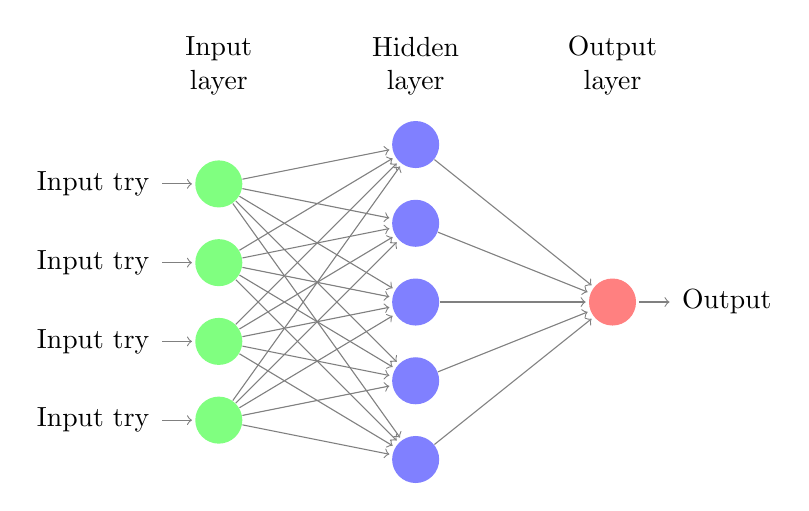
\begin{tikzpicture}[shorten >=1pt,->,draw=black!50, node distance=\layersep]
    \tikzstyle{every pin edge}=[<-,shorten <=1pt]
    \tikzstyle{neuron}=[circle,fill=black!25,minimum size=17pt,inner sep=0pt]
    \tikzstyle{input neuron}=[neuron, fill=green!50];
    \tikzstyle{output neuron}=[neuron, fill=red!50];
    \tikzstyle{hidden neuron}=[neuron, fill=blue!50];
    \tikzstyle{annot} = [text width=4em, text centered]

    % Draw the input layer nodes
    \foreach \name / \y in {1,...,4}
    % This is the same as writing \foreach \name / \y in {1/1,2/2,3/3,4/4}
        \node[input neuron, pin=left:Input try] (I-\name) at (0,-\y) {};

    % Draw the hidden layer nodes
    \foreach \name / \y in {1,...,5}
        \path[yshift=0.5cm]
            node[hidden neuron] (H-\name) at (\layersep,-\y cm) {};

    % Draw the output layer node
    \node[output neuron,pin={[pin edge={->}]right:Output}, right of=H-3] (O) {};

    % Connect every node in the input layer with every node in the
    % hidden layer.
    \foreach \source in {1,...,4}
        \foreach \dest in {1,...,5}
            \path (I-\source) edge (H-\dest);

    % Connect every node in the hidden layer with the output layer
    \foreach \source in {1,...,5}
        \path (H-\source) edge (O);

    % Annotate the layers
    \node[annot,above of=H-1, node distance=1cm] (hl) {Hidden layer};
    \node[annot,left of=hl] {Input layer};
    \node[annot,right of=hl] {Output layer};
\end{tikzpicture}
\end{center}

\newpage 

\addcontentsline{toc}{section}{References}

\bibliographystyle{alpha}
\bibliography{banknote_forgery_bib}
\end{document}
